\chapter{Design}
In this chapter we focus on how to implement what we have specified in the analysis chapter.
First, we describe our application's architecture.
Then, we discuss what technologies were considered for implementing the application, and which of the technologies were chosen and why.
We name our application "Choose well".

\section{Architecture}
\todo[inline]{add footnote}
We design our solution(footnote - from now on we will refer to the whole application as the solution as not to  confuse it with the applications it consists of) as multiple independent single-page applications for better modularity. 
One application is the guest dietary profile editor.
It allows a guest to set their dietary preferences like being allergic to something or being vegetarian.
Another application is the restaurant menu maker.
It serves for restaurant employees to specify their menu's contents.
Last application is the personalized menu viewer for restaurant guests.
It combines information gathered by the other applications to display personalized menus to guests. 
\todo[inline]{add figure number}
\todo[inline]{move bottom border a bit lower}
Figure x contains a depiction of our solution's architecture.

\begin{figure}[h]
  \centering
  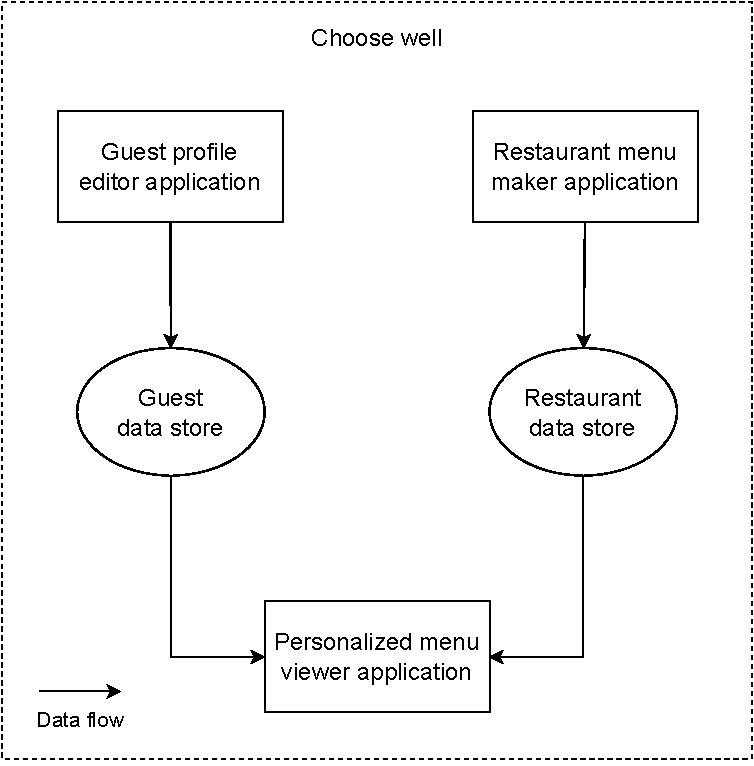
\includegraphics[width=0.62\linewidth]{master-thesis/img/architecture_data_flow.pdf}
  \caption{The solution's architecture}
\end{figure}

\section{Technological stack}
\todo[inline]{add links to technologies - footnotes, link to documentation of the technology}
There are various options out there for what technologies we can use to implement our application.
This section contains an overview of available tools and which ones we chose and why.

\subsection*{User interface}
  We need a UI so that a user can interact with the application.
  We need to be able to create an interactive user interface.
  We need to have state for logged in user.
  We need to fetch data from the internet.
  We need to integrate with Solid.

  Nowadays, there are many frameworks for building web applications.
  The most popular options are Angular, React and Vue.

  Angular is a platform and framework for building single-page client applications using HTML and TypeScript. 
  It implements its core and optional functionality as a set of TypeScript libraries. 
  The basic building blocks of the Angular framework are Angular components that are organized into \emph{NgModules}. 
  NgModules collect related code into functional sets; an Angular application is defined by a set of NgModules.

  React is a JavaScript library for rendering user interfaces.
  Applications written in React are built from modular and reusable pieces called components.
  React components receive data and return what should appear on the screen. 
  They can be passed new data in response to an interaction, like when the user types into an input. 
  React will then update the screen to match the new data.
  A notable feature is the use of a virtual Document Object Model, or Virtual DOM. 
  React creates an in-memory data-structure cache, computes the resulting differences on a re-render, and then updates the browser's displayed DOM efficiently. 
  This selective rendering provides a major performance boost.

  Vue is a JavaScript framework for building user interfaces. 
  It builds on top of standard HTML, CSS, and JavaScript and provides a declarative and component-based programming model.
  Vue uses an HTML-based template syntax that allows programmers to declaratively bind the rendered DOM to the underlying component instance's data.
  Under the hood, Vue compiles the templates into highly-optimized JavaScript code. 
  Combined with the reactivity system, Vue can intelligently figure out the minimal number of components to re-render and apply the minimal amount of DOM manipulations when the app state changes.

  We decide to choose \textbf{React} for developing the UI of our application.
  One of the reasons for this decision is that Solid is written for React.
  There exists a Solid React SDK which can help us to work with some of the core Solid principles.
  Ract also allows us to work with components as functions.
% end of \subsection

\subsection*{Programming language}
  We need to implement the application.

  As for programming languages, we considered two options. 
  JS, TS

  JavaScript is a lightweight, interpreted, or just-in-time compiled programming language with first-class functions. 
  It is most well-known as the scripting language for Web pages. 
  JavaScript is a prototype-based, multi-paradigm, single-threaded, dynamic language, supporting object-oriented, imperative, and declarative---e.g. functional programming styles.

  TypeScript is a superset of JavaScript. 
  It provides features such as optional static typing, classes, interfaces, and generics. 
  The goal of TypeScript is to help catch mistakes early through its type system and make JavaScript development more efficient. 
  One of the big benefits is enabling IDEs to provide a richer environment for spotting common errors as the programmer types their code.

  The goal is to make as few bugs during development as possible and that is why we decide to go with \textbf{Typescript}.
  Defining types of variables makes the code more readable to other developers.
% end of \subsection

\subsection*{Build tool}
  We need to create the application.
  We need to make the application to a single file that is sent to the client.
  We need to build and deploy our application.

  We considered Vite and Create React App

  Vite (French: [vit], like "veet") is a local development server written by Evan You and used by default by the Vue project templates. It has support for TypeScript and JSX.

  It monitors files as they're being edited and upon file save the web browser reloads the code being edited through a process called Hot Module Replacement (HMR) which works by just reloading the specific file being changed using ES6 modules (ESM) instead of recompiling the entire application.

  Vite is a newer build tool that has gained popularity in recent years. It was created to address the limitations of existing build tools, particularly in the development phase. Vite is a build tool that is optimized for speed. It leverages the latest browser technologies, such as ES modules and native browser imports, to provide fast build times.

  Vite is particularly useful for small to medium-sized projects that do not require complex configurations. It is built on top of the Rollup bundler, which is known for its fast build times. Vite also provides a development server that is optimized for performance. The server leverages HTTP/2 server push, which enables the server to send multiple responses for a single client request.

  Create React App is built on Webpack and Babel and it is a popular tool that enables developers to quickly set up a React project. It is an officially supported tool by the React team, making it a reliable choice. It creates a basic React application with all the necessary configuration files, dependencies, and scripts. The tool provides a pre-configured environment that abstracts away much of the configuration that developers would typically have to handle manually. This means that the developer can focus on writing code rather than configuration files.

  We chose \textbf{Vite} because it is better for deployment process

% end of \subsection

\subsection*{Deployment}
\todo[inline]{add link to GH Pages doc}
  For deployment, only \textbf{GitHub Pages} was considered.

  GitHub Pages is a static site hosting service that takes HTML, CSS, and JavaScript files straight from a repository on GitHub, optionally runs the files through a build process, and publishes a website.

  There are three types of GitHub Pages sites: project, user, and organization. Project sites are connected to a specific project hosted on GitHub, such as a JavaScript library or a recipe collection. User and organization sites are connected to a specific account on GitHub.com.

% end of \subsection

\subsection*{Package manager}
  We need a tool to manage our application's dependencies.
  A package manager can seamlessly handle installing and uninstalling of packages which is another name for JavaScript libraries.

  For package management in our application we consider two options: npm and yarn.

  npm is a package manager for the JavaScript programming language.
  npm is used to fetch any packages that an application needs for development, testing, and/or production, and may also be used to run tests and tools used in the development process.
  It consists of a command line client, also called npm, and an online database of packages, called the npm registry. 
  The registry is accessed via the client, and the available packages can be browsed and searched via the npm website.

  A successful and popular alternative package manager is Yarn. 
  Yarn resolves the dependencies using a different algorithm that can mean a faster user experience.
  More specifically, yarn can download packages in parallel to maximize network utilization.

  Although Yarn is just as good as npm for handling packages, the latter is more widely used.
  For this reason we decide to use \textbf{npm} for our application. 
% end of \subsection

\subsection*{Responsive design}
  Responsive web design or RWD is a web design approach to make web pages render well on all screen sizes and resolutions while ensuring good usability.
  We need our application to be responsive to various device screens.
  We want a mobile-first approach as most people use smartphones these days.
  The chosen tool should be well documented for ease of use.

  Two options were considered, which are Bootstrap, Material UI.
  Let us briefly introduce them.

  Made by myself and Jacob Thornton, Bootstrap is an open-source front-end toolkit created to help designers and developers quickly and efficiently build awesome stuff online. Our goal is to provide a refined, well-documented, and extensive library of flexible design components built with HTML, CSS, and JavaScript for others to build and innovate on.

  The most prominent components of Bootstrap are its layout components, as they affect an entire web page. The basic layout component is called "Container", as every other element in the page is placed in it.

  Once a container is in place, other Bootstrap layout components implement a CSS Flexbox layout through defining rows and columns.

  Material Design is a design language which uses grid-based layouts, responsive animations and transitions, padding, and depth effects such as lighting and shadows.

  The main purpose of Material Design is the creation of a visual language that combines principles of good design with technical and scientific innovation. 

  Designers optimize users' experience with 3D effects, realistic lighting and animation features in immersive, platform-consistent GUIs.

  We decide to opt for \textbf{Bootstrap} as it is easier to use and well documented.
% end of \subsection

\subsection*{Persistence}
Our application needs to store and later read data.
We decide to use the \textbf{Solid} technology for this purpose. 

\subsection*{Documentation}
\todo[inline]{add links to docs in footnote}
We need to capture how our application works for users and future developers.
Programmer documentation is available as several simple HTML pages created using \textbf{GitHub markdown}.
User documentation is in a form of a webpage which is hosted on \textbf{GitHub Pages}.

\subsection*{Authentication}
For authentication purposes, the Inrupt's solid-client JavaScript library is used.
We also use the Inrupt's React SDK which contains a Login component which uses the aforementioned library implicitly.

\todo[inline]{add testing}
% \subsection*{Testing}
% We need to test our application in order to prevent bugs during implementation.
% % https://legacy.reactjs.org/docs/testing-environments.html
